\documentclass[11pt, a4paper]{article}

% --- Packages ---
\usepackage[utf8]{inputenc}
\usepackage[T1]{fontenc}
\usepackage{lmodern}
\usepackage{geometry}
\geometry{margin=0.85in}
\usepackage{xcolor}
\usepackage{enumitem}
\usepackage{titlesec}
\usepackage{microtype}
\usepackage{tabularx}
\usepackage{booktabs}
\usepackage[most]{tcolorbox}
\usepackage{tikz}
\usetikzlibrary{positioning, arrows.meta}
\usepackage{xurl}
\usepackage{hyperref}
\hypersetup{colorlinks=true, urlcolor=primaryBlue, linkcolor=primaryBlue}

% --- Custom Colors ---
\definecolor{primaryBlue}{RGB}{10, 80, 160}
\definecolor{lightGray}{RGB}{245, 245, 245}

% --- Section Styling ---
\titleformat{\section}{\large\bfseries\color{primaryBlue}}{}{0em}{}[\titlerule]
\setlist[itemize]{leftmargin=*, noitemsep, topsep=2pt}
\setlist[enumerate]{leftmargin=*, noitemsep, topsep=2pt}
\setlength{\parindent}{0pt}
\setlength{\emergencystretch}{2em}

% --- Custom Box for Student Info ---
\newtcolorbox{studentbox}{
    colback=lightGray,
    colframe=primaryBlue,
    boxrule=0.5pt,
    arc=4pt,
    left=15pt,
    right=15pt,
    top=10pt,
    bottom=10pt
}

\begin{document}

% --- Header Section ---
\begin{center}
    {\huge \bfseries \color{primaryBlue} Dataset Datasheet} \\[0.2cm]
    {\large \textbf{Course:} DSPRO2 HS26} \\[0.1cm]
\end{center}

\vspace{0.4cm}

% --- Student & Project Information ---
\begin{studentbox}
    \begin{tabularx}{\textwidth}{l X}
        \textbf{Project Name:} & RentLens: Predicting Rents in Switzerland \\
        \textbf{Student Names:} & Elias Martinelli, Timo Schlumpf (Team 6) \\
        \textbf{Date:} & \today \\
        \textbf{GitHub Repository:} & \url{https://github.com/0xff4b/dspro2} \\
        \textbf{Scraper:} & \url{https://github.com/Elias-Martinelli/comparis-actor} \\
    \end{tabularx}
\end{studentbox}

\vspace{0.5cm}

% --- Section 1: Overview ---
\section{Dataset Overview}
\begin{itemize}
    \item \textbf{Official Name:} RentLens Comparis Listings, October 2026.
    \item \textbf{Owner / Contact:} Collected by Team 6 at HSLU. The listings are taken from comparis.ch, where the offers of most Swiss portals (Homegate, ImmoScout24, immobilier.ch among others) appear in one search. We have no data agreement with Comparis.
    \item \textbf{Short Description:} All flats and houses that were advertised for rent or for sale on comparis.ch between 26 and 29 October 2026, 65{,}552 listings in total. Each listing carries the price, the number of rooms, the living area, the address, the coordinates and the description text. On top of that come building data from the federal register of buildings (GWR), location data from geo.admin and the tax burden of the municipality.
    \item \textbf{Version \& Date:} v1.0, scraped 26--29 October 2026.
    \item \textbf{Reference:}
    \begin{itemize}
        \item Source: \url{https://www.comparis.ch/immobilien}
        \item Scraper code: \url{https://github.com/Elias-Martinelli/comparis-actor}
        \item Scraper on Apify: \url{https://console.apify.com/actors/E4hkR2fhfBFkfFwiZ/info/readme?build=latest}
        \item DSPRO1 datasheet (rentumo.ch, April 2026): \texttt{docs/archive/dspro1/data-sheet/}
    \end{itemize}
\end{itemize}

% --- Section 2: Motivation ---
\section{Motivation and Intended Use}
\begin{itemize}
    \item \textbf{Primary Purpose:} This datasheet belongs to the DSPRO2 module at HSLU. Our DSPRO1 data from rentumo.ch was too small for the questions we had in mind (9{,}405 listings) and it came without any description text. For DSPRO2 we needed a larger sample, coverage of the whole country and the texts themselves.
    \item \textbf{Intended Use:} The main task is a regression: predict the monthly net rent in CHF from the features of a listing. As an extension we fit the same models to the for-sale listings and predict the purchase price. The predictions are what the RentLens app shows, once as a fair-rent check and once on a price map.
    \item \textbf{Out-of-Scope Use:} Legal rent assessment (Art.\ 269 ff.\ OR), tenant screening, credit or mortgage decisions, and passing on or selling the listings.
\end{itemize}

% --- Section 3: Composition ---
\section{Composition and Coverage}
\begin{itemize}
    \item \textbf{Data Types:} Relational tables in SQLite. Almost every column is a number or a category; the only free text is the listing description, written in German, French or Italian depending on where the flat is. Image links are stored, the images themselves are not used.
    \item \textbf{Population:} Flats, houses and single rooms in all 26 cantons, provided they were online during the scrape and had at least one photo.
    \item \textbf{Dataset Size:} 65{,}552 listings, 25{,}879 of them for rent and 39{,}673 for sale. Cleaning and merging leave 19{,}571 rental objects and 28{,}476 objects for sale. After cleaning, 1{,}537 municipalities are still in the data (DSPRO1 had 1{,}186).
    \item \textbf{Known Gaps / Imbalances:}
    \begin{itemize}
        \item We only see asking rents. The rents in existing contracts are usually lower and do not appear on the portals.
        \item Only listings that came with a photo made it into the data.
        \item 41\,\% of the rentals give no side costs, so net and gross rent cannot be separated for them.
        \item 23\,\% of the rentals have no living area.
        \item Some listings carry only the coordinate of the village, not of the building.
        \item Coverage in the small cantons (AI, NW, OW, UR) is thin, with very few listings.
    \end{itemize}
\end{itemize}

% --- Section 4: Collection ---
\section{Sources and Collection}

\textbf{Data pipeline}

\vspace{0.4em}
\begin{center}
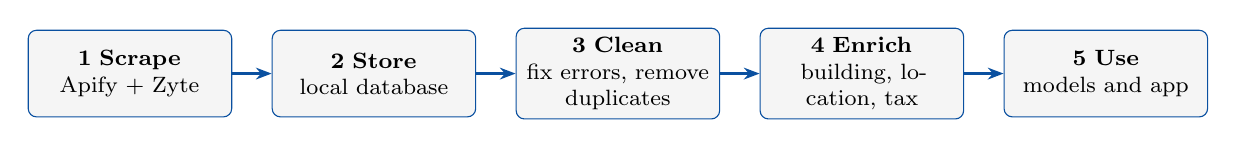
\begin{tikzpicture}[
    node distance=0.5cm,
    stage/.style={draw=primaryBlue, fill=lightGray, rounded corners=3pt, align=center,
                  font=\footnotesize, minimum height=1.1cm, text width=2.35cm},
    arrow/.style={-{Stealth[length=2mm]}, primaryBlue, thick}]
    \node[stage] (scrape) {\textbf{1 Scrape}\\Apify + Zyte};
    \node[stage, right=of scrape] (store) {\textbf{2 Store}\\local database};
    \node[stage, right=of store] (clean) {\textbf{3 Clean}\\fix errors, remove duplicates};
    \node[stage, right=of clean] (enrich) {\textbf{4 Enrich}\\building, location, tax};
    \node[stage, right=of enrich] (use) {\textbf{5 Use}\\models and app};
    \draw[arrow] (scrape) -- (store);
    \draw[arrow] (store) -- (clean);
    \draw[arrow] (clean) -- (enrich);
    \draw[arrow] (enrich) -- (use);
\end{tikzpicture}
\end{center}

\begin{enumerate}
    \item \textbf{Scrape.} Our scraper (\href{https://github.com/Elias-Martinelli/comparis-actor}{comparis-actor}) runs on \href{https://console.apify.com/actors/E4hkR2fhfBFkfFwiZ/info/readme?build=latest}{Apify}. Comparis stops a search after 1{,}000 results, so the scraper queries every canton several times with different price ranges to get around that limit. The listing pages are loaded through the \href{https://www.zyte.com/zyte-api/}{Zyte API} because Comparis blocks bots, and every listing is opened once so that all fields can be read from the page. E-mail addresses and phone numbers are removed while the text is collected, which means the contact details of the advertisers never reach the database. The scraper also keeps track of the listings it has already saved, so a stopped run continues where it stopped and no listing ends up in the database twice.
    \item \textbf{Store.} The results are downloaded from Apify into a single local database file (\texttt{data/raw/}\allowbreak\texttt{comparis.db}). Nobody edits that file; every later step reads from it and writes its output somewhere else.
    \item \textbf{Clean.} Placeholder values are corrected first: construction year 0, a living area of ``1\,m\textsuperscript{2}'', 999 rooms and similar entries that only fill a field. Then we keep only the rentals that have a monthly price. Since the same flat is usually advertised on several portals, one object shows up several times in the scrape, and we merge those copies into a single object. Objects outside a plausible range (10 to 500\,m\textsuperscript{2}, CHF 300 to 15{,}000 per month) are dropped.
    \item \textbf{Enrich.} Public sources are joined on the cleaned listings: construction year and building size from the GWR, public transport quality, sun and population from geo.admin, and the tax burden of the municipality from the ESTV (more on that below). The descriptions serve one purpose, and that is repairing fields. When rooms, area, floor, lift, balcony or renovation year are missing or wrong, the value is read out of the text; the text itself does not go into the models.
    \item \textbf{Use.} The cleaning notebook writes the one clean database, and the models and the app read only that database. Listings that do not survive cleaning stay in the table together with the reason for their removal, so the numbers below can be traced back.
\end{enumerate}

\vspace{0.4em}
\textbf{How many listings are left after cleaning}

\vspace{0.2em}
\begin{center}
\small
\begin{tabular}{lr}
    \toprule
    Step & Listings \\
    \midrule
    Scraped (rent and sale) & 65{,}552 \\
    Rentals with a monthly price & 25{,}666 \\
    After merging duplicates & 23{,}129 \\
    After removing implausible values & 19{,}571 \\
    \bottomrule
\end{tabular}
\end{center}

\vspace{0.4em}
\textbf{Tax as a new feature.} After the mid-term presentation the tax burden of the municipality became a feature in the price models. The reasoning is that the same flat is worth more in a place where people keep more of their income, so the local tax rate should absorb part of the location effect. The values come from the ESTV table ``Tax burden in the municipalities'' (\url{https://www.estv.admin.ch/de/steuerbelastung-in-den-gemeinden}): cantonal, municipal and church tax as a percentage of income, for every municipality.

\vspace{0.4em}
\textbf{Cost.} The scrape has cost about USD 58 so far, USD 22 for Zyte and USD 35.84 for Apify, and that figure already contains all the test runs. A weekly update that only fetches new listings costs about USD 1 to 3.

\vspace{0.4em}
\textbf{Tools for analysis.} For the work on the descriptions we are also looking at \href{https://console.typesafe.ai}{TypeSafe AI}, which was recommended to us. It answers in a fixed schema and returns a confidence score with each answer, which is what a task like ``read the missing floor out of this description'' actually needs. Nothing in the pipeline uses it yet.

\begin{itemize}
    \item \textbf{Provenance:} Public listing pages of comparis.ch (third party); open government data from swisstopo, BFS, ARE, BFE and ESTV.
    \item \textbf{Collection Method:} Web scraping with Apify and the Zyte API; public APIs and downloads for the extra data.
    \item \textbf{Jurisdictions:} Switzerland, all 26 cantons.
\end{itemize}

% --- Section 5: Labels ---
\section{Labels and Targets}
\begin{itemize}
    \item \textbf{Target Definition:} The monthly net rent in CHF, meaning the rent without side costs. For the sale listings the target is the purchase price in CHF.
    \item \textbf{Labeling Process:} There is no manual labelling step. The price is the one the landlord or the agency wrote into the listing, and the scraper reads it from the price field of the page.
    \item \textbf{Quality Control:} Listings without a price are removed and the price is never guessed, since an imputed target would only teach the model our own assumption. Prices per m\textsuperscript{2} that fall far outside the usual range are flagged and checked by hand. Prices that appear inside a description are masked, otherwise a text model could read the target straight out of the text.
\end{itemize}

% --- Section 6: Data Quality Audit ---
\section{Quality Assessment (Data Audit)}
\begin{itemize}
    \item \textbf{Preprocessing Steps:} Placeholder values are fixed, rooms stay as half rooms (3.5), coordinates are converted to LV95, duplicates are merged, the public data is joined, and missing fields are filled from the description where that is possible.
    \item \textbf{Initial Audit Findings:}
    \begin{itemize}
        \item About 10\,\% of the rental listings are copies of another listing.
        \item A few entries under ``rent'' were really sale prices, up to CHF 2.4 million. They are removed.
        \item For about 80\,\% of the rentals we found the building in the GWR.
    \end{itemize}
    \item \textbf{Quality Dimensions:}
    \begin{itemize}
        \item \emph{Completeness:} rent, area, rooms and location have to be present; a listing that misses one of them is dropped.
        \item \emph{Accuracy:} value ranges, outlier flags and the comparison with the GWR.
        \item \emph{Consistency:} the same format as the DSPRO1 data, with cantons as two-letter codes such as ZH or BE.
        \item \emph{Timeliness:} a snapshot from the end of October 2026; whatever changes on the portals afterwards is not in the data.
    \end{itemize}
\end{itemize}

% --- Section 7: Ethics & Governance ---
\section{Legal, Ethical, and Governance}
\begin{itemize}
    \item \textbf{Sensitive Data:} The dataset contains no data about tenants. The scraper removes e-mail addresses and phone numbers, and the cleaning step masks names, links and amounts inside the descriptions. The address of a flat is only used to find its building.
    \item \textbf{Compliance:} The terms of use of comparis.ch do not allow automated scraping, and in DSPRO1 Comparis told us that scraping needs their approval. We have no approval. The data therefore stays inside the course: the raw files sit on our own machines and are not in the GitHub repository, and what we publish are results, models and figures. Swiss data protection law (nFADP) applies, and we keep only the fields the project needs.
    \item \textbf{Consent \& Licensing:} No licence was granted for the listings. The public data is open government data and can be used freely as long as the source is cited. OpenStreetMap data is under the ODbL.
\end{itemize}

% --- Section: Structure & Schema ---
\section{Dataset Structure and Schema}
\begin{itemize}
    \item \textbf{File Formats:} SQLite databases, Parquet and CSV files.
    \item \textbf{Directory Layout:}
    \begin{itemize}
        \item \texttt{data/raw/}: scraped data, unchanged
        \item \texttt{data/interim/}: cleaned data
        \item \texttt{data/external/}: public geodata
        \item \texttt{notebooks/}: cleaning, models, QoLI
    \end{itemize}
    \item \textbf{Schema Summary:} The clean database has three main tables: \texttt{listings} (every scraped listing together with the reason why it was removed, if it was), \texttt{rent} (one row per rental object) and \texttt{buy} (one row per object for sale).
    \item \textbf{Units \& Encodings:} Prices in CHF, rent per month, areas in m\textsuperscript{2}, coordinates in LV95, cantons as two-letter codes.
\end{itemize}

% --- References ---
\section{References}
\begin{itemize}
    \item Comparis real estate: \url{https://www.comparis.ch/immobilien}
    \item Scraper code: \url{https://github.com/Elias-Martinelli/comparis-actor}
    \item Scraper on Apify: \url{https://console.apify.com/actors/E4hkR2fhfBFkfFwiZ/info/readme?build=latest}
    \item Zyte API: \url{https://www.zyte.com/zyte-api/}
    \item Project repository: \url{https://github.com/0xff4b/dspro2}
    \item GWR building register: \url{https://www.gwr.admin.ch/de/data/supply/public_content.html}
    \item geo.admin API: \url{https://api3.geo.admin.ch}
    \item ESTV tax burden: \url{https://www.estv.admin.ch/de/steuerbelastung-in-den-gemeinden}
    \item swissBOUNDARIES3D: \url{https://www.swisstopo.admin.ch/de/landschaftsmodell-swissboundaries3d}
    \item TypeSafe AI: \url{https://console.typesafe.ai}
\end{itemize}

\end{document}
